\documentclass[a4paper,10pt]{article}

\usepackage[margin=2cm]{geometry}
\usepackage{graphicx}
\usepackage{amsmath}
\usepackage{array}
\usepackage{hyperref}
\usepackage[all]{hypcap}
\usepackage{listings}
\lstdefinestyle{TerminalStyle}{
  language=bash,
  basicstyle=\small\sffamily,
  numbers=left,
  numberstyle=\tiny,
  numbersep=3pt,
  frame=tb,
  columns=fullflexible,
  linewidth=0.9\linewidth,
  xleftmargin=0.1\linewidth
}
\lstdefinestyle{HtmlStyle}{
  language=html,
  basicstyle=\small\sffamily,
  numbers=left,
  numberstyle=\tiny,
  numbersep=3pt,
  frame=tb,
  columns=fullflexible,
  linewidth=0.9\linewidth,
  xleftmargin=0.1\linewidth
}
\lstdefinestyle{OutputStyle}{
  language=html,
  basicstyle=\small\sffamily,
  frame=tb,
  columns=fullflexible,
  linewidth=0.9\linewidth,
  xleftmargin=0.1\linewidth
}

\setlength{\parindent}{0pt}
\setlength{\parskip}{1ex plus 0.5ex minus 0.2ex}
\title{
\includegraphics[width=12cm]{Eeufeeslogo.jpg} \\
       Department of Computer Science \\
       University of Pretoria \\
       \vspace{0.5cm}
       Software Engineering\\
       COS301 Main Project \\
       \vspace{0.5cm}
       \begin{large} \textbf{Team CodeX}\\ ReRoute Systems\end{large}}

\date{} 
\author{	Bondjobo, Jocelyn 		13232852 		\\
		Malangu, Daniel		13315120		\\
		Kirker, Tim			11152402		\\
		Hammond, Eunice	NK	13222563		\\
		Burgers, Heinrich		15059538		\\
}

\begin{document}
\maketitle
\thispagestyle{empty}
\clearpage

\newpage
\pagenumbering{roman}
\thispagestyle{empty}
\tableofcontents
\clearpage

\newpage
\pagenumbering{arabic}

\section{Introduction}

	\subsection{Background} 
	Reroute Systems is a software company with different in-house developed applications. The Purchase Management System application is the main application and is mainly active in the pharmaceutical space. The main functionality of this system is routing of requests for products from account holders to various wholesalers/suppliers, receiving the result of the order and routing the answer back to account holder.
	
	\subsection{Purpose} 	
	For an account holder to request a product, s/he must search for it against the database with all the product information. The challenge is that each wholesaler/supplier can name/describe the product in a different way/manner, and when the account holder performs the search against the master product list, the same product must be displayed across all wholesalers/suppliers, using the link between master product list and the different wholesaler's/supplier's product list.
	
	\subsection{Scope} 
	The core of the system is a search engine which is enriched with functionality
of performing some machine learning in order to retrieve the product in a master file found in a database running on the server through RESTful calls. The high level modules and their responsibilities are shown in the figure below. \\ \\

	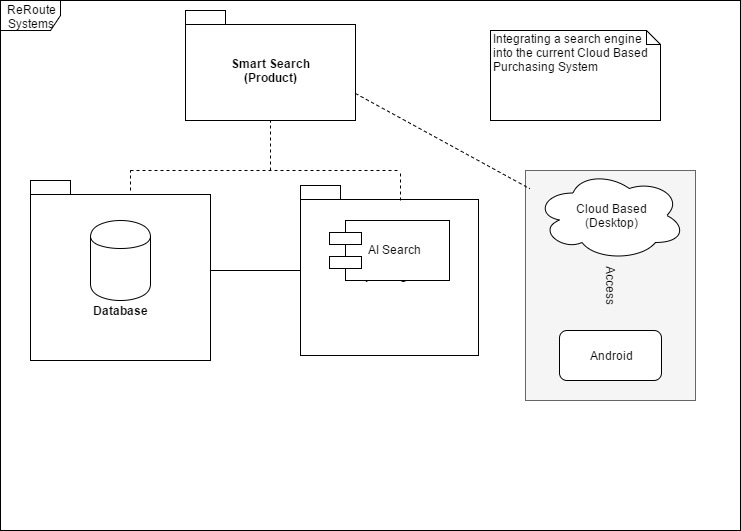
\includegraphics[scale=0.60]{scope1.jpg}
	\subsection{Definitions, Acronyms, and Abbreviations} 

	\begin{itemize} 
	\item Cloud-based: Refers to applications, services or resources made available to users on demand via the Internet from a cloud computing provider's servers.
	\item Android: A Linux based operating system developed by Google Inc. and the Open Handset Alliance for smart phones, tablets, and other mobile computing devices. Android applications are developed in Java.
	\item REST: Representational State Transfer. It is a architectural pattern consisting of guidelines and best practices
for creating scalable web services.
	\item HTTP: HyperText Transfer Protocol, standardised by RFCs 7230-7237.
	\end{itemize}
	
	\subsection{References} 
	(To be completed)
	
	\subsection{Stakeholders}
	The stakeholders of the system include the following,
	\begin{itemize}
	\item \textbf{The Client} is Diederik Mostert, Software Director of ReRoute Systems who proposed the project as a result of a challenge faced in the company, which is to search a product on master file with different combinations used by each wholesaler.
	\item \textbf{Users in Pharmaceutical space.} They will use the system to retrieve information of the product they need.
	\end{itemize}

	\newpage

\section{Overall Description}

\subsection{Technologies}{
	The following are technologies used in this project:
	\begin{itemize}
		\item SOAP
		\item ZIZO database
		\item Reddis
		\item Firebird
		\item WDSL (Web Service Definition Language)
		\item GlassFish
		\item JUnit
		\item JMeter
		\item XML
		\item Pathway
	\end{itemize}
}
	
\subsection{Product Perspective}
        \subsubsection{System Interface}{
			\begin{enumerate} 
				\item User Interface:
					\begin{itemize}
				\item Functionality:\\
					The functionality of the user interface is to allow the user to interact with the system. Through this aspect of the system, the user can perform all the functions necessary to use the efficient search of the system. Through this, the user is able to specify the search criteria to be used by the system.\\
				\item How functionality achieves requirements:\\	
					The user interface allows the functionality of the application to meet the requirements. The user is able to search for any product based on any value they enter in, such as the product name or product ID. The user is able to view displayed information of products, that is based closely on keywords and values or any thing resembling the name. \\
					\end{itemize}
					
				\item Hardware Interface:
					\begin{itemize}
					\item Functionality:\\
					The functionality of this system interface is the physical hardware that allows software operation. The hardware in this case is specifically the desktop which allows the user to run the system.\\
				\item How functionality achieves requirements:\\
					This hardware will allow the achievement of the requirements by facilitating the operation of the application. The networking hardware of the components such as the Wireless Fidelity infrastructure or LAN connections between the devices, will allow for communication to the system server.
				\end{itemize}
				
				\item Software Interface:
					\begin{itemize}
					\item Functionality:\\
						The functionality of the software interface is to facilitate the communication between the hardware infrastructure of the device(s) running the application's front-end and the Reroute Server. An example of this would be the operating system of the device in use. The operating system would allow the application to make use of the networking infrastructure and communicate the necessary information to the application via RESTful calls. This would enable the device to communicate with the server and perform the necessary requests.\\

					\item How functionality achieves requirements:\\
The above functionality would allow the achievement of the requirements, as the communication of the application with the system server is vital to the operation of the search. By allowing communication over WI-Fi, the user is able to communicate with the server from any location, or just stick to older and more familiar devices such as desktop computers, fulfilling the requirement.
					\end{itemize}
			\end{enumerate} 
}

		
            \subsubsection{User Interface}
	    All users will be able to use the management system and search aspect from their desktop devices when the application is launched.
For the account user interface, the registered users will be able to login to their account, using their account information.
\\
	    \subsubsection{Communications Interface}
	 \begin{itemize}
	    \item Users using the web will use HTTP/HTTPS protocol.
	    \item RESTful calls from the different platforms to the server API.
	    \item Cloud-based server running the database.
	    \end{itemize}
	    
            \subsubsection{Memory}
	    {The desktop application will use a minimum amount of space of roughly 300MB.\\
		Primary memory(RAM) will use 50MB on average, based on how long the application is being used.}
		
            \subsubsection{Operations}

            	{A series of operations will be required to be fulfilled by the system. The user will use the system in cases that comprise of searching any of the different properties of a product. The user may also search for a product based on the name of the product of interest.\\\\
            	The system will provide a user the option to either save their data, such as variations of product names, locally on the device or remotely on the server.}
		
           \subsubsection{Sit Adaption Requirements}
        (to be completed)

		\subsection{Product Functions} {The main function of the search will be to retrieve product information based on the values given to the system. The functions of the system will include:  }
	\begin{itemize}
  		\item A search-based on a specific property of a product such as the name or ID.
		\item The use of a dictionary to link related words, thus enhancing the search.
	\end{itemize}
	
    	\subsection{User Characteristics}  

{The general user will use the system to retrieve product information. They will require minimal skills in order to utilise the application, including the ability to connect to the Wi-Fi and use it. They will require background knowledge/education in the medical or pharmaceutical field to use the application.\\}

    	\subsection{Constraints}
	The system will:
	\begin{itemize}
		\item only use the data contained in the client's existing database.
	The system is subjected to working with an internet connection due to the linkage with the cloud. Without this in place, the system will not function.	
		
	\end{itemize}
	
    	\subsection{Assumptions and Dependencies}
	Users will:	
	\begin{itemize}
		\item have some form of pharmaceutical background knowledge.
		\item have basic computer skills.
		\item be connected to an internet connection.
	\end{itemize}

	The database will be updated regularly.

	\newpage
	\section{Architecture Requirements}
	This section discusses the requirements that surround the software infrastructure.

	\subsection{Access Channel Requirements}
		\subsubsection{Human Access Channels}
	This element must allow for desktop applications to give the user access to the search.
	It will also be based on the client-side of the Cloud-based architectural pattern.

		\subsubsection{System Access Channels}
	All system access will be made over a uniform interface which will assist in faster development time, ease of maintenance and 		lower overall cost associated with the system. The common interface that will be used will be a RESTful API. All client-side 		interaction will be done via the User Interface which will in turn use the RESTful API set of the system to accomplish the given 	task.
	
	\subsection{Architecture Constraints}
	\begin{itemize}
		\item Representational State Transfer (REST) will be used. It is an architectural style used to design networked 	applications, and depends on cacheable and stateless client-server and communications protocols, using the HTTP protocol in most cases. 
		\item Service Oriented Architecture (SOA). The concept of service is based on SOA. It makes it easier for software components on computers that are over a network to work together with no need to make changes to the underlying program itself. 
		\item Cloud-based Architecture will also be used. This architecture is a model which consists of a front-end platform (client), back-end platform (servers), a cloud based delivery, and a network (Internet). Combined, these components make up cloud computing architecture.
		\item Unit Testing to automate the following tasks: Compilation of Java code, running test cases and generating product documentation.
	\end{itemize}
	
	\subsection{Architectural Patterns}
	\subsubsection{Cloud-based Architectural Pattern}
	This architecture consists of front-end, back-end, cloud-based delivery, and a network.
	Our system is combined with the client as front-end, the database and servers, and the network. 
	Regarding the delivery platform, Reroute makes use of the Software as a Service(SaaS) service-model. This model involves
	the cloud provider installing and maintaining software in the cloud and users running the software from their cloud clients
	over the Internet. It is scalable, which yields a major plus as our system is required to return results at a very high rate.\\
	
	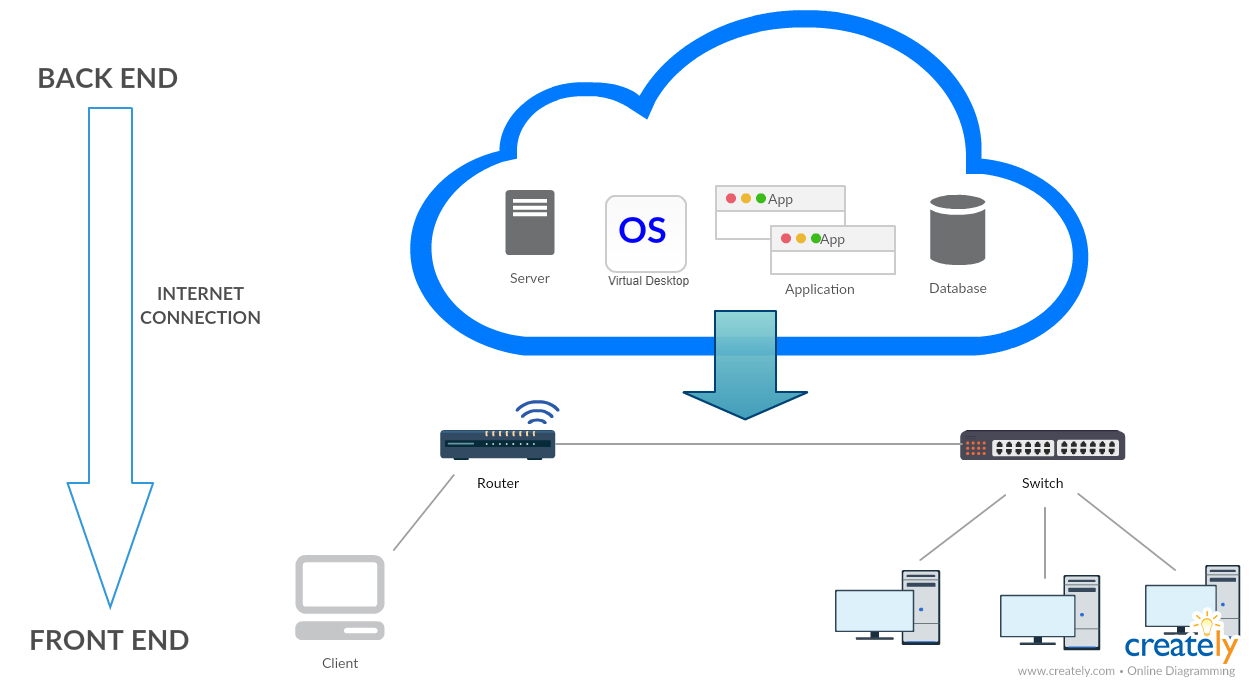
\includegraphics[scale=0.4]{Diagrams/Cloud-based Architecural Diagram.jpg}\\

	\subsubsection{Representational State Transfer (REST) Architectural Pattern}
	REST is an architectural pattern for designing networked applications.

The Uniform interfaces is combined of resource names and HTTP, GET, DELETE, POST, PUT.
A REST service is:
\begin{itemize}
	\item Language-independent (C-sharp can communicate to Java, etc.),
	\item Can be used with firewalls,
	\item Platform-independent (MAC, Windows, UNIX) and
	\item Standards-based (runs on top of HTTP)
\end{itemize}

	\subsubsection{Services Orientated Architecture/ Microservices Architecture}
An architectural pattern in software design in which system use cases are divided into one or more service operations, and these service operations are then implemented, either individually or combined with other service operations, by a reusable SOA service. The SOA architecture itself comprises of five layers:
	\begin{enumerate}
		\item Consumer interface: The GUI for end users accessing application services
		\item Business process: The representation of system use cases
		\item Services: The consolidated inventory of all available services.
		\item Service components: The reusable components used to build the services, such as functional libraries.
		\item Operational system: Contains data repository, technological platforms, etc.
	\end{enumerate}
 	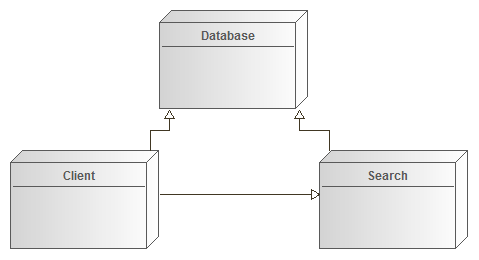
\includegraphics[scale=0.5]{service_oriented_architecture_diagram.png}\\

Not to be confused with an API, this architectural pattern provides an aggregated collection of service which implement the use cases of the system. The user or developer themselves can choose which of these available services to call on. This architectural pattern was chosen because it is built around the principles of decoupling modules. Service objects must be decoupled from one another and can be distributed on different machines and implemented using different technologies, but implement a single interface, and communicate with one another using well defined interfaces, either locally or over a network. This also lends itself well to system reliability and scalability. More than one system provider may be used, enabling the system to switch to another service provider should one fail, or instantiating more service providers if system load increases.

	
	\newpage
	\section{Specific Requirements}
This section gives a detailed description of the system requirements. It describes all the functional as well as the quality requirements of the system.

	\subsection{External Interface Requirements}

            \subsubsection{Software Interfaces}
The smart search application being build will be designed to run on Desktop running Windows OS.

	\subsection{Requirements}
	\subsubsection{Functional Requirements} 
		\begin{itemize}
		\item Fuzzy Search: This program must be able to locate and return products that are related to the searched term. It should be able to return the same product if various ways of writing the name is used.
	
		\item Fast Run-time:\\
			Because there are very large amounts of data to be searched, it is vital for the program to be very efficient.  Even though this could be a non-functional requirement, it is vital for this program to be as fast and efficient as possible.
			
		\item Machine Learning:\\
			The ability to learn from a user's previous interaction and adapt to it will improve the system’s capability and ability greatly. This can be done by using the dictionary provided by the ZIZO database, for creating new links between products that appear seemingly unrelated.\\
	
		\item Handle Concurrent Users:\\
			This program will be used by many people, in many different fields simultaneously. It is therefore very important for it to be able to handle multiple users at the same time. This will be achieved by the Cloud-based architecture.
	
		\item Scalability:\\
			Since it is essential for this system to be efficient with large datasets as well as small datasets, scalability will be an essential functional requirement. The system’s ability to stay efficient with very large sets of data is an essential part to the system.
		 \end{itemize}

	\subsubsection{Non-Functional Requirements}
		\begin{itemize}
		\item Predictive Typing:\\
			Predictive typing is when the program suggests a possible solution as the user is typing. This is often based on previous searches and most common searches. This will help improve the user experience. 
		
		\item Spell checker:\\
			The program will check the spelling as the user is typing a product name to enhance the search. 

		\item Roubstness:\\
			The system will not be easily breakable as it will be error proof to a feasible extent, to avoid unnecessary fault and not wholly be affected by the hardware failures. The system should be able to recover quickly from such failures, or at least be able to hold up or return to a valid stage/state.
			
			
		\item Reliability:\\
			This product should be able to adapt to different users in various fields as well as to different habits, interfaces, environments and needs of users.  
	
		\item Storing and using search history:\\
			Being able to store the search history will increase the user experience, help with predictive typing and improve the program's ability to learn and adapt.\\
		\end{itemize}

	
	\subsubsection{Use Case Prioritization} 
		 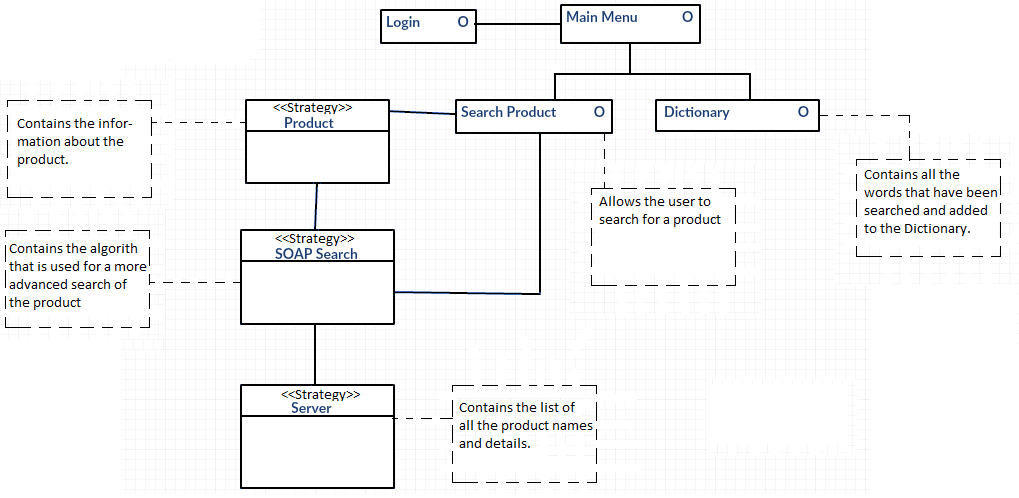
\includegraphics[scale=0.62]{Diagrams/ClassDiagramUpdatedWithDesign.png}\\
		\begin{enumerate} 
		\item \textbf{Critical} 
		\begin{itemize}
		\item Create User
		\item View and Edit User
		\item Authenticate User which includes Login/Logout and Permissions
		\item Edit Data
		\item Search Data
		\end{itemize}
		
		\begin{itemize} 
			\item Login
			 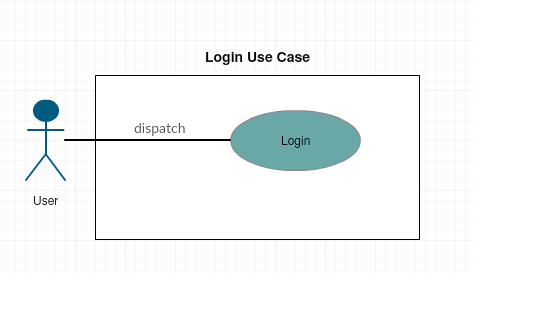
\includegraphics[scale=0.62]{Diagrams/Login Use Case.png}\\
		 
			\item Search Product \\
			\begin{itemize}
				\item Pre-condition(s): The user has to have been logged in successfully.  \\
				\item Post-condition(s): System returns possible matches, or search not found. \\
 				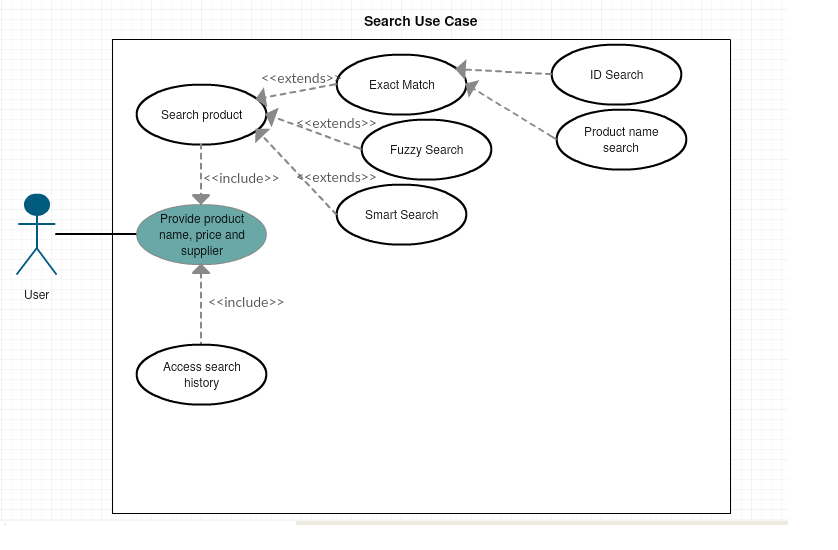
\includegraphics[scale=0.35]{Diagrams/Search Use Case.png}
			\end{itemize}
			
			\item Logout\\
			
\includegraphics[scale=0.5]{Diagrams/logout.png}\\

			\item{Register User}
				\begin{itemize}
					\item Description:
				This use case will be used by the customers to register themselves as users of the system. This is required before they are allowed to login. 
				This will be created a user of the system.

					\item Pre-Conditions:
					\begin{enumerate}
						\item The user doesn't exist on the system.
						\item The user has provided all the required details.
						\item All the details provided by the user a valid. 
					\end{enumerate}
					\item Post-Conditions
					\begin{enumerate}
						\item The user will be created as a user of the system.
					\end{enumerate}
	 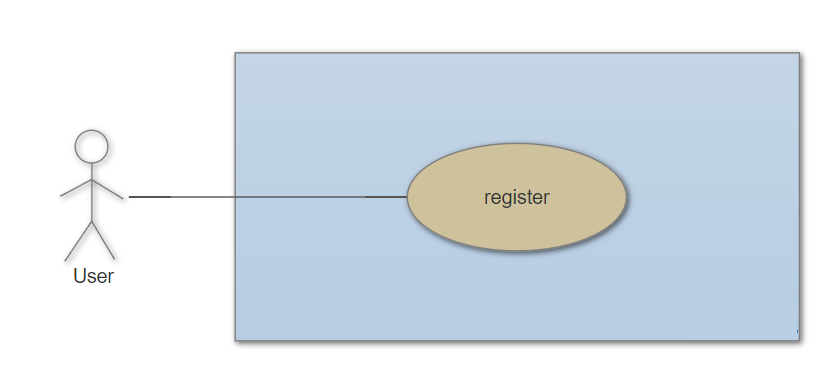
\includegraphics[scale=0.62]{Diagrams/RegisterUseCase.png}\\
				\end{itemize}


				\item View/Edit User
				\begin{itemize}
					\item Description
						\begin{enumerate}
							\item This case will be used by the customers to view and edit their profile details.
						\end{enumerate}
					\item Pre-Condition:
						\begin{enumerate}	
							\item The customer must be logged in.
							\item All the edited details need to be valid.
						\end{enumerate}
					\item Post-Condition:
						\begin{enumerate}
							\item The customer's details will be edited.
							\item The customer must be able to see his/her details.
							\item The database keeping the customer's details has to be updated.
						\end{enumerate}
	 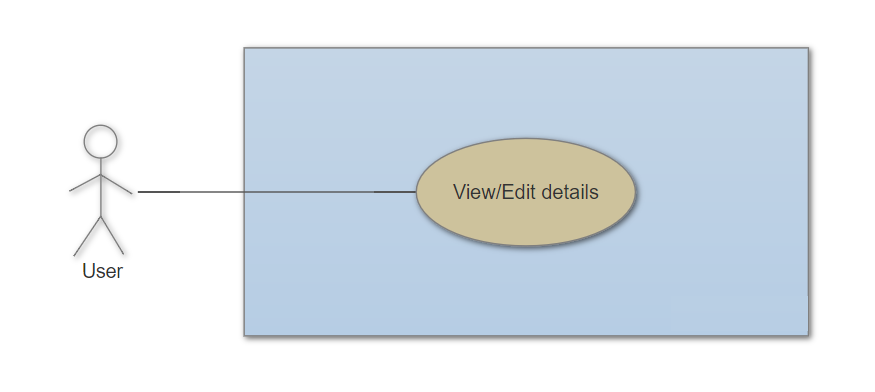
\includegraphics[scale=0.62]{Diagrams/View_EditUseCase.png}\\
				\end{itemize}
			\item Manipulate Data to the database
			\begin{itemize}
				\item Description
					\begin{enumerate}
						\item The develop/administative user will use this use case to add, remove and edit data on the database. 
					\end{enumerate}
				\item Pre-Condition:
					\begin{enumerate}	
						\item The administative user needs to be logged in to the system. 
					\end{enumerate}
				\item Post-Condition:
					\begin{enumerate}
						\item The database will be updated with the new information. 
					\end{enumerate}
		 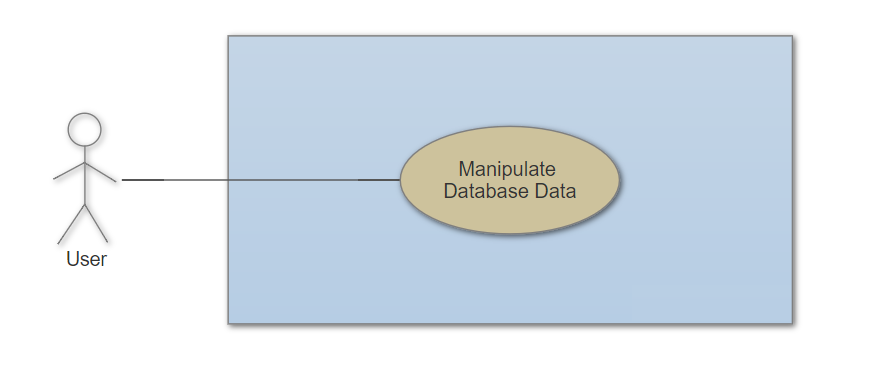
\includegraphics[scale=0.62]{Diagrams/ManipulateDatabaseUseCase.png}\\

			\end{itemize}
			\item Manipulate Data in Dictionary
			\begin{itemize}
				\item Description
					\begin{enumerate}
						\item The administative users will use this use case to add data to the dictionary. This will improve the accuracy of the search function.
					\end{enumerate}
				\item Pre-Condition:
					\begin{enumerate}	
						\item The user is logged in as adminitrative user.
						\item The linked words must be identified as a match.
						\item The user must be familier with the format of the dictionary.
					\end{enumerate}
				\item Post-Condition:
					\begin{enumerate}
						\item New words are linked in the dictionary.
						\item The search will be more accurate.
					\end{enumerate}
		 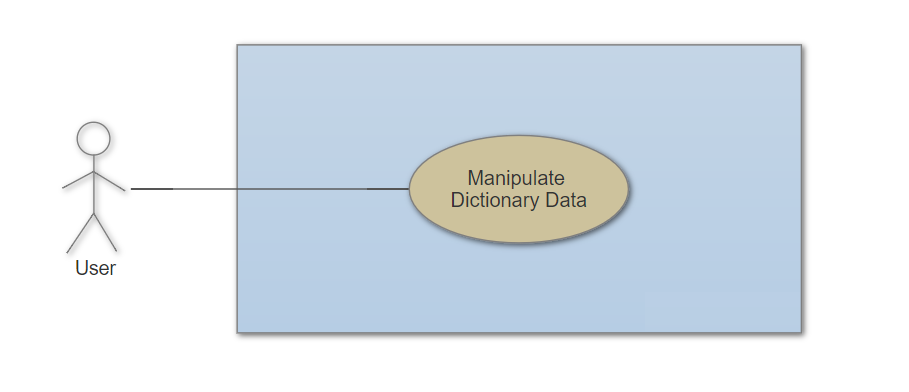
\includegraphics[scale=0.62]{Diagrams/ManipulateDictionaryUseCase.png}\\
		\end{itemize} 
		
		\item \textbf{Important} 
		\begin{itemize}
                \item The application must search for the item the user enters for their desired search. 
                \item The system must return all possible matches to whatever the user searches.
		\item The system must perform a smart search.
		\item The application must be fast.git 
		\item Smart searches
                \end{itemize}
		
		\item \textbf{Nice to have}
		\begin{itemize}
		\item System using a search history, predictive typing. 
		\item A mobile version of the system such as Android.
		\item Remember Search History
		\item Mobile Application

		\end{itemize}
\end{itemize}
		\end{enumerate} 
	
	\subsection{Application Design}
	\subsubsection {Activity Diagram}
		 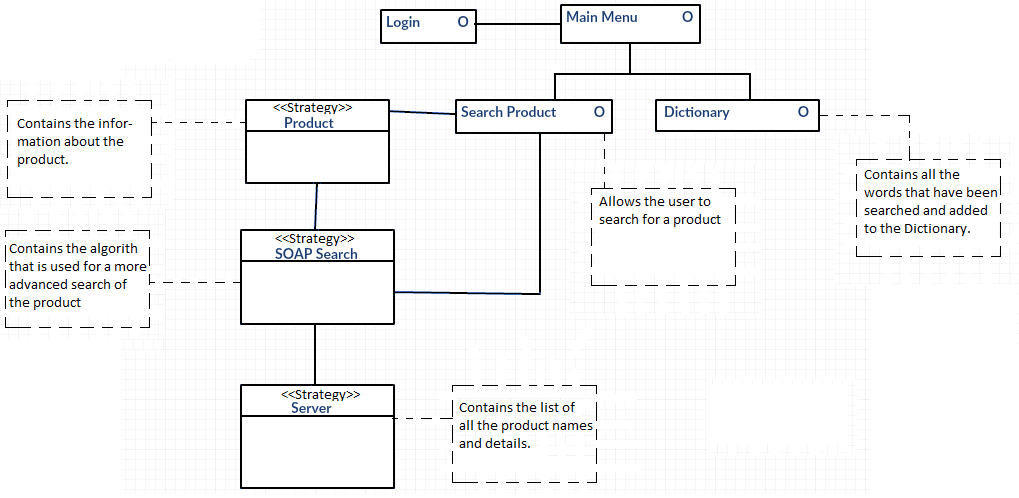
\includegraphics[scale=0.62]{Diagrams/ClassDiagramUpdatedWithDesign.png}\\
		 
	\subsubsection {Sequence Diagram}
		 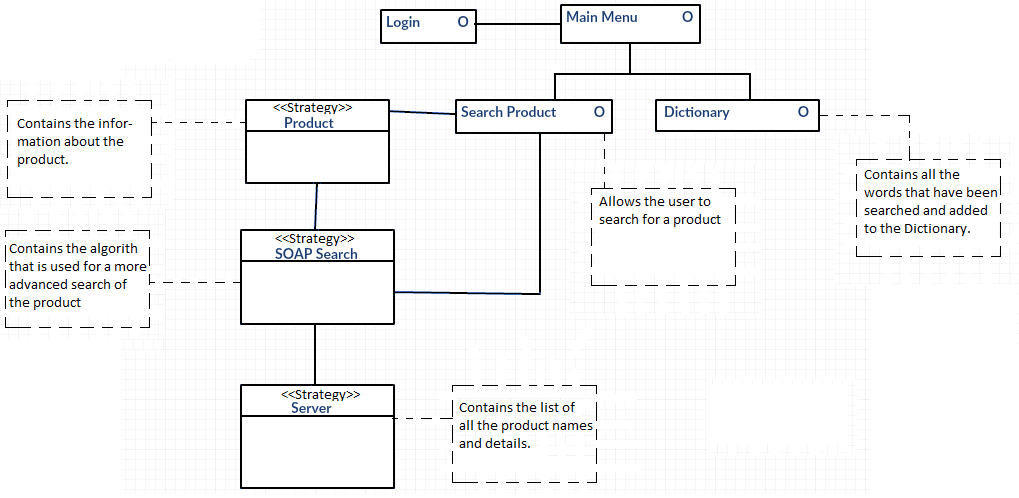
\includegraphics[scale=0.62]{Diagrams/ClassDiagramUpdatedWithDesign.png}\\
	
	\subsubsection {Deployment Diagram}
		 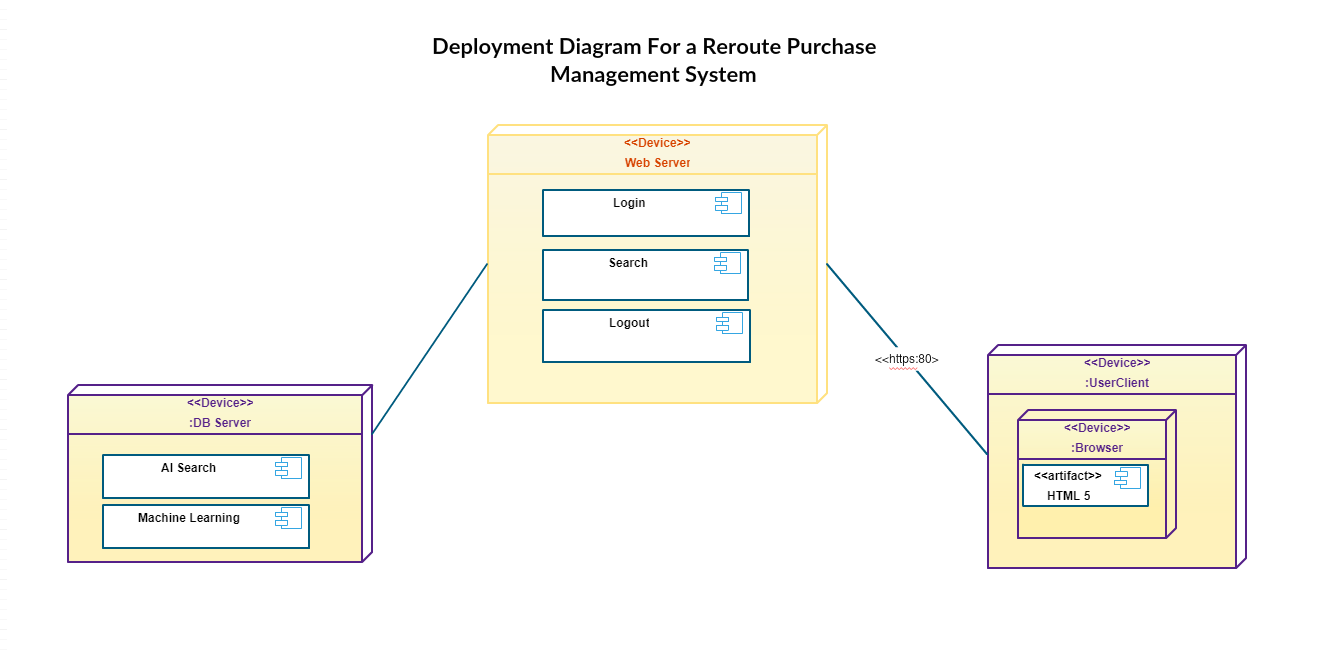
\includegraphics[scale=0.62]{Diagrams/Deployment Diagram.png}\\
		
		
	\subsection{Performance Requirements}
	The performance requirements of the smart search app. can be sub-divided into two components, of which are the following:
	\begin{itemize}
	\item Client Application:
		\begin{itemize}
		\item The software needs to be responsive and lightweight enough to run well on desktop.
		\item During User search, the Smart Search system will need to perform in real time showing results as necessary.
		\item The data usage should be kept to a minimum as to not overload the whole system's Wi-Fi infrastructure being used for non-searching purposes.\\
		\end{itemize}

	\item Server Performance Requirements:
		\begin{itemize}
		\item The system should be able to handle multiple users using the smart search.
		\item The system has to be able run at a high speed, returning the results of a search immediately.
		\item The system should be able to handle a capacity of requests made to the database to make efficient searches and matches. 
		\item The system should be able to return matches of a high probability of available data in the database on the cloud.
		\item The system will need to be able to concurrently handle smart searches across the board.
		\end{itemize}
	\end{itemize}

	\subsection{Design Constraints}
	\begin{itemize}
		\item to be completed
	\end{itemize}

	\subsection{Software System Attributes}
	The software system will have the following attributes:
		\begin{itemize}
		\item Availability: The system and its functions will be available to any registered user as long as there is an internet connection. 
		\item Reliability: The system will provide results that are available on the database to match whenever a user performs a search/smart search.
		\item Portability: The system will be able to function across a multiple interfaces. Therefore, it will be able to port to Android and iOS with ease at a later time, if it is made available for mobile.   
		\item Maintainability: The application will be able to be extended easily with new functionality. There will also be a good test environment to reduce and make it easy to find system errors.  
		\item Robustness: The system will be able to stand against errors made by users in the search, returning no results and error messages as a result.
		\end{itemize}
        
	\subsection{Other Requirements}

\subsubsection{Quality requirements}
(to be completed)




\clearpage

\section{Open Issues}
\subsection {GitHub Repository}

\includegraphics[width=12cm]{CodeX_logo.jpg} \\
Team CodeX Repository: \url{https://github.com/josephbondjobo/CodeX}

This repository contains:
\begin{itemize}
\item All work done by team members.
\end{itemize}



\newpage
\clearpage
\addcontentsline{toc}{section}{References}

\end{document}
